\section{ENCODE data} \label{encode-data-sect}
The Encyclopedia of DNA Elements (ENCODE) project \citep{Dunham2012} is an international collaboration of research groups with diverse backgrounds and expertise in production and analysis of NGS genomic data. \emph{Fig. \ref{encode-seq-pic}} shows only some examples of the different platforms and techniques that are used from ENCODE to measure diverse biological components in order to interpret the human genome. That is, to discover functional elements in the genome, including genes, transcripts, transcriptional regulatory regions, chromatin structure and DNA methylation patterns.

\begin{figure}[!ht]
\begin{center}
 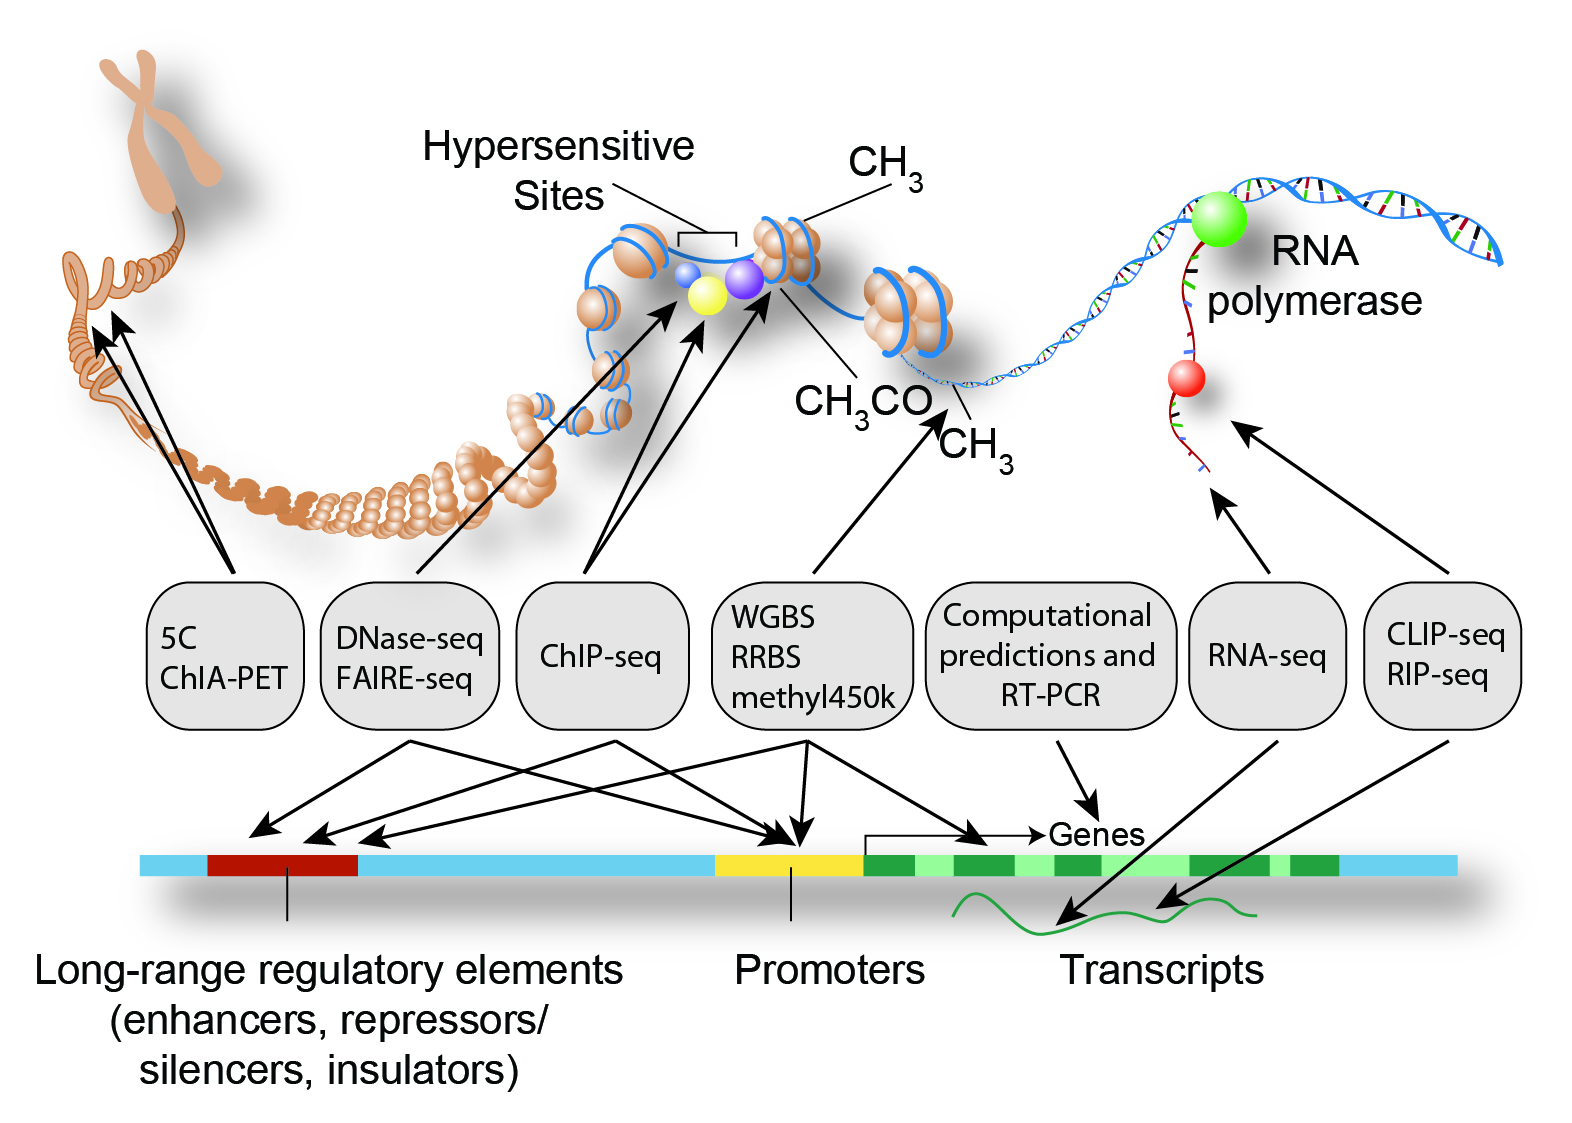
\includegraphics[scale = 0.25]{images/encode-seq.png}
\caption{\emph{Some of the XX-Seq techniques used from the ENCODE projet. Credits: Darryl Leja (NHGRI), Ian Dunham (EBI), Michael Pazin (NHGRI) \citep{Dunham2012}.}}
\label{encode-seq-pic}
\end{center}
\end{figure} 

To evaluate our proposed methods, Tier 1 cells (\ie high priority) from the ENCODE project are used. These data are released to the public through a web accessible database (\emph{http://genome.ucsc.edu/ENCODE/}) and can be visualised through the \emph{UCSC Genome Browser} at the same web portal. More specifically, the cell types that will be studied are the immortalized cell lines, K562, coming from a human female with chronic myelogenous leukemia, and the human embryonic stem cells, H1-hESC, coming from a human male \citep{Dunham2012}.

%This project is mainly concentrated in modelling and analysing transcriptome and DNA methylation data generated from NGS technology.